\subsection{Obstacle avoidance : exploration with left and right recursive search}
Before the competition of 2024, the team has implemented a new obstacle avoidance algorithm which has
proven to be effective at low driving speeds. This section will go in detail about how the implementation works.

When the robot encounters an obstacle in its path, it initiates a pathfinding algorithm to explore alternative routes. This exploration phase involves adjusting the robot’s direction by incrementally rotating the vector facing the target, to the left and to the right, until a free angle is identified. The exploration tree is a binary tree with a branch going to the left and the other to the right of the robot.

\paragraph{Obstacle Detection and Rotation}

Upon detecting an obstacle, the robot begins exploring by rotating incrementally in one direction (e.g., left). After each small rotation, it evaluates whether the new direction results in a clear path of a short length. The robot checks if any obstacles intersect the trajectory.

Free Angle: If no obstacles block the path, the angle is marked as “free,” and the robot proceeds along this trajectory.

Obstacle Detected: If an obstacle remains, the robot continues rotating further in the same direction (left or right) until a free path is found or the maximum angle limit is reached.

\paragraph{Recursive Exploration}

When a free path is identified, the algorithm recursively evaluates the next step from the new position. It continues checking whether this position brings the robot closer to the target while considering any new obstacles in its way. The exploration process repeats until the target is reached or the maximum itteration number is reached.

\paragraph{Trajectory Smoothing}

Once a path is calculated, it is smoothed to eliminate unnecessary waypoints, retaining only significant points to optimize the trajectory.

\paragraph{Optimal Direction Selection}

If both left and right explorations yield free paths, the algorithm selects the optimal path based on proximity to the target. If no fully clear path is found, the robot moves along the trajectory that gets it closest to the target.

\paragraph{Continuous Recalculation}

The algorithm runs continuously, recalculating the best trajectory in real-time, ensuring dynamic responsiveness to changing environments.


\paragraph{Pros}
\begin{itemize}
    \item Adaptability: Continuously adjusts to dynamic environments.
    \item Incremental Exploration: Ensures precise obstacle avoidance.
\end{itemize}

\paragraph{Cons}
\begin{itemize}
    \item Computational Cost: Recursive processing can be resource-intensive.
    \item Inefficiency: The algorithm may fail to find a path within the iteration limit.
\end{itemize}

\subsubsection{Comparison with Informed RRT*}
This obstacle avoidance algorithm has proven to be sufficient in practice. To compare its performance, we have decided to implement
a modification of the Informed RRT* algorithm described by team KIKSbot \cite{tdp_kiksbot_2023}. Since RRT* is a popular choice in the SSL communinity,
choosing this algorithm seems to form a good comparison basis.

The Informed RRT* search was performed over 800 iterations, but because of its stochastic nature, a path might not be found
during these steps. So the search has been run 20 times in order for the algorithm to give us the best result and lowest-path cost.
Observing the results of both search algorithms, depicted in figures \ref{fig:own-obs-avoid} and \ref{fig:informed-rrt-star}.
Cost of a path is defined as the cumulative distance of each point in the path. Note that no smoothing was performed on the Informed RRT* result.

\begin{figure}[h]
    \centering
    \begin{subfigure}[c][][c]{0.4\linewidth}
        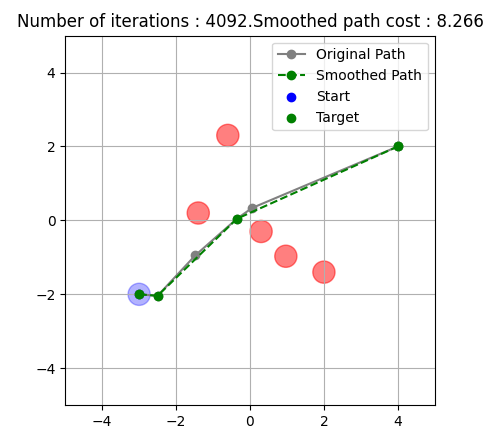
\includegraphics[scale=0.5]{rstar}
        \caption{Binary-tree based search}
        \label{fig:own-obs-avoid}
    \end{subfigure}
    \hfill
    \begin{subfigure}[c][][c]{0.4\linewidth}
        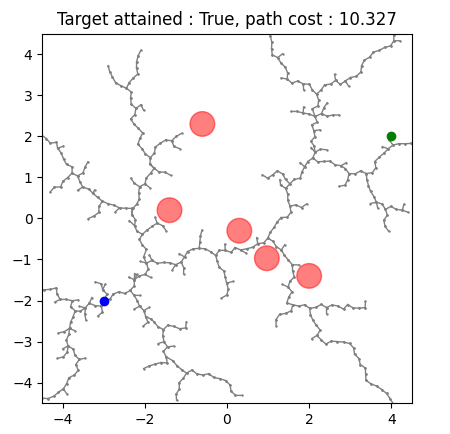
\includegraphics[scale=0.5]{informed_rrt}
        \caption{Informed RRT* square search}
        \label{fig:informed-rrt-star}
    \end{subfigure}
    \label{fig:avoidance}
    \caption{Comparison of our own obstacle avoidance algorithm against Informed RRT*. Both axis represent the x and y coordinates.
    Informed RRT*. Parameters: step distance $d_{step} = 0.15$, and distance to check whether target is attained : $d_{attained} = 0.25$.
    The start and target points are respectively in blue and green,
    and grey points in the Informed RRT* graph represent the resulting tree generated.}
\end{figure}